\documentclass[11pt]{article}
\usepackage[a4paper,margin=1in]{geometry}
\usepackage{amsmath,amssymb,amsthm}
\usepackage{tikz}
\usepackage{xcolor}
\usepackage{booktabs}
\usepackage[hidelinks]{hyperref}
\hypersetup{pdftitle={A randomized Pascal triangle whose average blows up},pdfauthor={Vamshi Jandhyala}}
\setlength{\parskip}{0.4em}
\setlength{\parindent}{0pt}

\newtheorem{theorem}{Theorem}
\newtheorem{lemma}{Lemma}
\newtheorem{corollary}{Corollary}
\theoremstyle{remark}
\newtheorem*{remark}{Remark}

\newcommand{\E}{\mathbb{E}}
\definecolor{heads}{RGB}{0,70,200}
\definecolor{tails}{RGB}{200,30,30}

\title{A randomized Pascal triangle whose average blows up}
\author{Vamshi Jandhyala}
\date{}

\begin{document}
\maketitle
\vspace{-2em}

\begin{abstract}
Build Pascal's triangle, but let each interior entry be the sum of the two entries above it with probability $p$ and their absolute difference otherwise. For which $p$ does the expected average of all the entries tend to infinity? This was known for $p>1/2$. We show that the expected sum of row $n$ is at least $\lambda(p)^n$ with $\lambda(p)=p^2+\sqrt{p^4+4p(1-p)}$, which exceeds $1$ exactly when $p>1-1/\sqrt2\approx0.293$. The proof rests on one observation: the sum grows only if the row is rough, and the randomness keeps it rough. A computer-assisted extension of the same idea reaches $p\ge 0.232$. Both arguments are formally verified in Lean, the second relative to an exactly checked finite certificate.
\end{abstract}

\section{The question}

Write $1$s down both sides of a triangle. For each interior position flip a coin that shows heads with probability $p$. On heads write the sum of the two numbers above; on tails write the absolute value of their difference. Here is a sample with $p=1/3$, heads in blue and tails in red:
\[
\begin{array}{c}
1\\
1\quad 1\\
1\quad \textcolor{heads}{2}\quad 1\\
1\quad \textcolor{tails}{1}\quad \textcolor{tails}{1}\quad 1\\
1\quad \textcolor{tails}{0}\quad \textcolor{heads}{2}\quad \textcolor{tails}{0}\quad 1\\
1\quad \textcolor{tails}{1}\quad \textcolor{tails}{2}\quad \textcolor{tails}{2}\quad \textcolor{tails}{1}\quad 1\\
1\quad \textcolor{heads}{2}\quad \textcolor{heads}{3}\quad \textcolor{tails}{0}\quad \textcolor{tails}{1}\quad \textcolor{tails}{0}\quad 1
\end{array}
\]
Dan asked on Mathematics Stack Exchange~\cite{MSE} and then on MathOverflow~\cite{MO} for the limit
\[
L_p=\lim_{N\to\infty}\E\bigl[\text{arithmetic mean of all the numbers in rows }0,1,\dots,N-1\bigr].
\]
At $p=1$ the triangle is Pascal's and $L_1=\infty$. At $p=0$ every entry is the parity of the binomial coefficient in the same place, because $a+b$ and $|a-b|$ have the same parity; odd binomial coefficients have density zero, so $L_0=0$. In between, simulations are hard to read. Large values arise rarely, then dominate the average, and runs of a few thousand rows can look settled when they are not.

\emph{Before reading on, try the first step.} Why must $L_p$ be infinite when $p>1/2$?

Einar R{\o}dland's answer~\cite{Rodland} gives the reason. A new entry is at least $p$ times the sum of its parents in expectation, and each old entry is a parent of two new entries, so the expected row sum is multiplied by at least $2p$ at every step. For $p\le1/2$ this bound is useless, and the question stayed open. The bound throws away the tails outcome entirely. The point of this note is that the tails outcome cannot be thrown away, because it carries the growth whenever the row is rough.

Write $S_n$ for the sum of row $n$. Row $n$ has $n+1$ entries, so the first $N$ rows contain $N(N+1)/2$ numbers and the expected mean is $\frac{2}{N(N+1)}\sum_{n<N}\E S_n$.

\begin{theorem}\label{thm:A}
For $0<p\le1$ and every $n\ge0$,
\[
\E S_n\ \ge\ \lambda(p)^n,\qquad \lambda(p)=p^2+\sqrt{p^4+4p(1-p)} .
\]
The growth factor $\lambda(p)$ exceeds $1$ exactly when $2p^2-4p+1<0$, that is, when $p>1-1/\sqrt2\approx0.2929$. For such $p$, $L_p=\infty$.
\end{theorem}

At $p=1$ the bound is $2^n$, the exact row sum of Pascal's triangle. At $p=1/2$ it gives growth factor $(1+\sqrt{17})/4\approx1.28$, where the simple argument gave $1$.

\begin{theorem}\label{thm:B}
For $29/125\le p\le1$ and every $n\ge0$, $\E S_n\ge(5001/5000)^n$. Hence $L_p=\infty$ for $p\ge0.232$.
\end{theorem}

The proof of Theorem~\ref{thm:B} uses an exact finite computation, described in Section~\ref{sec:B}. Whether $L_p$ is finite for any $p>0$ remains open; Section~\ref{sec:open} collects what is known.

\section{Rough rows grow}

Pad each row with zeros on both sides. Then every entry, including the $1$s on the edges, comes from the same rule: from parents $0$ and $1$ both coins give $1$, and from two zero parents both give $0$. A row is now a sequence $x=(x_j)_{j\in\mathbb Z}$ of nonnegative numbers, finitely many nonzero, and the next row $x'$ has $x'_j$ built from the pair $(x_{j-1},x_j)$ with a fresh coin for each $j$.

Besides the sum $S(x)=\sum_j x_j$ we need the \emph{total variation}
\[
V(x)=\sum_j |x_{j+1}-x_j| ,
\]
which measures how rough the row is. For row $0$, the single entry $1$ between zeros, $S=1$ and $V=2$. In general $V\le 2S$, since $|x_{j+1}-x_j|\le x_{j+1}+x_j$.

\begin{lemma}\label{lem:S}
$\E[S(x')\mid x]=2p\,S(x)+(1-p)\,V(x)$.
\end{lemma}

The same computation for a single entry, written with $\min(a,b)$ in place of $|a-b|$, appears in a comment by user196574 on~\cite{MO}~\cite{comment}.

\begin{proof}
The new entry above the pair $(a,b)$ has mean $p(a+b)+(1-p)|a-b|$. Sum over all adjacent pairs: each $x_j$ lies in two pairs, which gives $2pS$, and each difference $|x_{j+1}-x_j|$ occurs once, which gives $(1-p)V$.
\end{proof}

Read the formula in two parts. The first term, $2pS$, is R{\o}dland's bound. The second is a bonus for roughness: every jump between neighbors is paid back with probability $1-p$. Three rows with the same sum $4$ show the effect.
\begin{center}
\begin{tabular}{lccc}
\toprule
row & $S$ & $V$ & $\E[S']$\\
\midrule
$1\ 1\ 1\ 1$ & $4$ & $2$ & $2+6p$\\
$1\ 2\ 1$ & $4$ & $4$ & $4+4p$\\
$2\ 0\ 2$ & $4$ & $8$ & $8$\\
\bottomrule
\end{tabular}
\end{center}
The flat row shrinks in expectation when $p<1/3$. The row with a hole in it doubles whatever the coins do: each $2$ next to a $0$ produces $2$ under either rule. So the question becomes whether the process keeps its rows rough. If the rows smoothed out, $V$ would be small compared with $S$ and the sum would decay for small $p$.

\section{Disagreeing coins make rows rough}

\begin{lemma}\label{lem:V}
$\E[V(x')\mid x]\ \ge\ 4p(1-p)\,S(x)-2p(1-p)\,V(x)$.
\end{lemma}

The right-hand side equals $4p(1-p)\sum_j\min(x_j,x_{j+1})$, because $\min(a,b)=\tfrac12(a+b-|a-b|)$. So the lemma says: wherever two neighbors are both large, the next row is likely to have a jump.

\begin{figure}[ht]
\centering
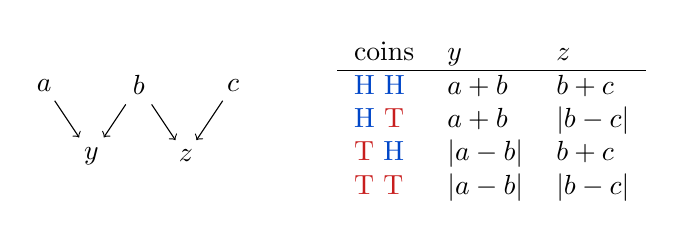
\begin{tikzpicture}[x=1.2cm,y=0.9cm]
\node (a) at (0,1) {$a$}; \node (b) at (1,1) {$b$}; \node (c) at (2,1) {$c$};
\node (y) at (0.5,0) {$y$}; \node (z) at (1.5,0) {$z$};
\draw[->] (a) -- (y); \draw[->] (b) -- (y); \draw[->] (b) -- (z); \draw[->] (c) -- (z);
\node[anchor=west,align=left] at (3,0.5) {
\begin{tabular}{lll}
coins & $y$ & $z$\\ \hline
\textcolor{heads}{H} \textcolor{heads}{H} & $a+b$ & $b+c$\\
\textcolor{heads}{H} \textcolor{tails}{T} & $a+b$ & $|b-c|$\\
\textcolor{tails}{T} \textcolor{heads}{H} & $|a-b|$ & $b+c$\\
\textcolor{tails}{T} \textcolor{tails}{T} & $|a-b|$ & $|b-c|$
\end{tabular}};
\end{tikzpicture}
\caption{Two neighboring new entries share the parent $b$. When the coins disagree, one entry is a sum and the other a difference, and the jump $|y-z|$ is large.}
\label{fig:coins}
\end{figure}

\begin{proof}
Take two neighboring new entries $y$ and $z$ with parents $(a,b)$ and $(b,c)$, as in Figure~\ref{fig:coins}. Keep only the two outcomes in which the coins disagree; each has probability $p(1-p)$, and the other two contribute something nonnegative. Then
\[
\E|y-z|\ \ge\ p(1-p)\Bigl(\bigl|(a+b)-|b-c|\bigr|+\bigl|(b+c)-|a-b|\bigr|\Bigr)
\ \ge\ p(1-p)\Bigl((a+b-|a-b|)+(b+c-|b-c|)\Bigr),
\]
using $|u|\ge u$ twice and regrouping. The last bracket is $2\min(a,b)+2\min(b,c)$. Summing over all neighboring pairs of new entries, each $\min(x_j,x_{j+1})$ appears twice, so
\[
\E[V(x')\mid x]\ \ge\ 4p(1-p)\sum_j\min(x_j,x_{j+1})=4p(1-p)\Bigl(S-\frac V2\Bigr). \qedhere
\]
\end{proof}

\section{Proof of Theorem~\ref{thm:A}}

Lemmas~\ref{lem:S} and~\ref{lem:V} are two linear inequalities in the pair $(S,V)$. Neither quantity grows on its own: $S$ needs $V$, and $V$ is fed by $S$ but drained by itself. A weighted combination can still grow. Try $F=S+tV$ with $t\ge0$. Since $S$ and $V$ are nonnegative,
\[
\E[F(x')\mid x]\ \ge\ \bigl(2p+4p(1-p)t\bigr)S+\bigl((1-p)-2p(1-p)t\bigr)V .
\]
We want the right-hand side to be $\lambda(S+tV)$ for a single factor $\lambda$, so we ask for
\begin{equation}\label{eq:eig}
2p+4p(1-p)t=\lambda,\qquad (1-p)-2p(1-p)t=\lambda t .
\end{equation}
The second equation gives $t=(1-p)/(\lambda+2p(1-p))$. Substituting into the first and clearing the denominator leaves
\[
\lambda^2-2p^2\lambda-4p(1-p)=0,
\]
whose positive root is $\lambda(p)$. With this $\lambda$ and $t$, which is positive for $0<p<1$ and zero at $p=1$, we have $\E[F(x')\mid x]\ge\lambda F(x)$ for every row $x$. Taking expectations over the first $n$ steps, one at a time,
\[
\E F(\text{row }n)\ \ge\ \lambda^n F(\text{row }0)=\lambda^n(1+2t).
\]
Finally $F\le(1+2t)S$ because $V\le2S$, so $\E S_n\ge\lambda^n$.

The growth factor exceeds $1$ when the quadratic $q(\mu)=\mu^2-2p^2\mu-4p(1-p)$, which is negative at $\mu=0$, is still negative at $\mu=1$, that is, when $1-2p^2-4p(1-p)=2p^2-4p+1<0$. The roots of $2p^2-4p+1$ are $1\pm1/\sqrt2$, so the condition is $p>1-1/\sqrt2$.

For the average, the sum over the first $N$ rows is at least its last term $\lambda^{N-1}$, while the number of entries is $N(N+1)/2\le N^2$. So the expected mean is at least $\lambda^{N-1}/N^2$, which tends to infinity when $\lambda>1$. This proves Theorem~\ref{thm:A}.

\begin{remark}
The pair \eqref{eq:eig} says that $(1,t)$ is a left eigenvector of the matrix of Lemmas~\ref{lem:S} and~\ref{lem:V}, with eigenvalue $\lambda$. The argument is the standard Lyapunov-function method for Markov chains, applied with the simplest pair of functions that see roughness.
\end{remark}

\section{Looking further along the row}\label{sec:B}

The weight $F=S+tV$ only sees neighbors. Lemma~\ref{lem:V} also discards the outcomes in which both coins agree, and those outcomes create jumps between entries two apart. Adding terms that see further gives a better bound. Theorem~\ref{thm:B} uses
\[
F=S+tV+uV_2+vW,\qquad V_2=\sum_j|x_{j+2}-x_j|,\quad W=\sum_j\bigl||x_{j+2}-x_{j+1}|-|x_{j+1}-x_j|\bigr|,
\]
with $t=\tfrac{1249}{2500}$, $u=\tfrac{3}{100}$, $v=\tfrac{557}{2500}$, and growth factor $\lambda=\tfrac{5001}{5000}$. Here $W$ measures how much the jumps themselves change, a second-order roughness. As before $V_2\le2S$ and $W\le V_2$, so $F\le KS$ with $K=1+2t+2u+2v$, and $F=K$ on row $0$.

The new difficulty is that $\E[F(x')\mid x]$ no longer splits into two clean formulas. Instead we reduce it to a statement about four consecutive entries. Each term of $F(x')$ involves at most three neighboring new entries, and these depend on four consecutive old entries and three coins. For $a,b,c,d\ge0$ let $y,z,w$ be the new entries above $(a,b)$, $(b,c)$, $(c,d)$, with independent coins, and set
\begin{align*}
I&=\tfrac14(a+b+c+d)+\tfrac t3\bigl(|a-b|+|b-c|+|c-d|\bigr)+\tfrac u2\bigl(|a-c|+|b-d|\bigr)\\
&\qquad+\tfrac v2\Bigl(\bigl||a-b|-|b-c|\bigr|+\bigl||b-c|-|c-d|\bigr|\Bigr),\\
O&=\tfrac13(y+z+w)+\tfrac t2\bigl(|y-z|+|z-w|\bigr)+u|y-w|+v\bigl||y-z|-|z-w|\bigr|,\\
G_p(a,b,c,d)&=\E\Bigl[O-\tfrac{81}{2500}(y+w-2z)\Bigr]-\lambda I+\tfrac{999}{10000}(a+d-b-c).
\end{align*}
Each term of $F$ involves one, two or three consecutive entries, and $I$ gives it the weight $1/k$ in each of the $k$ windows of four that contain it; $O$ does the same for the new row with windows of three. Summing over all windows along a zero-padded row, $\sum I$ is exactly $F(x)$ and $\sum O$ is exactly $F(x')$. The two correction terms add up to zero along any row, so they cost nothing: they move a little weight between neighboring windows. Hence $\E[F(x')\mid x]\ge\lambda F(x)$ follows by summation from the local inequality
\begin{equation}\label{eq:local}
G_p(a,b,c,d)\ \ge\ 0\qquad\text{for all }a,b,c,d\ge0.
\end{equation}

For fixed $p$, $G_p$ is homogeneous and piecewise linear in $(a,b,c,d)$. It is linear on each cell of an arrangement of hyperplanes through the origin: the coordinate hyperplanes; $a=b$, $b=c$, $c=d$, $a=c$, $b=d$, $a-2b+c=0$ and $b-2c+d=0$; and, for every choice of $y\in\{a+b,\pm(a-b)\}$, $z\in\{b+c,\pm(b-c)\}$, $w\in\{c+d,\pm(c-d)\}$, the hyperplanes $y=z$, $z=w$, $y=w$ and $y-2z+w=0$. (The equation $\bigl||y-z|-|z-w|\bigr|=0$ factors as $(y-w)(y-2z+w)=0$.) After removing repeats there are $41$. Each cell inside the nonnegative orthant is a pointed cone, generated by its extreme rays, and each extreme ray is the intersection of three independent hyperplanes of the arrangement. A linear function that is nonnegative on the generators of a cone is nonnegative on the whole cone, so it suffices to check \eqref{eq:local} on the $251$ such rays in the orthant. On each ray $G_p$ is a cubic polynomial in $p$, one degree for each coin. Writing it in the Bernstein basis on $[29/125,1]$~\cite{Farouki}, all $1004$ coefficients turn out to be positive rationals, the smallest being $3007/78125000$. A cubic with nonnegative Bernstein coefficients is nonnegative on the whole interval, so \eqref{eq:local} holds for every $p$ in the range and not only on a grid. A second certificate with $\lambda=51/50$ covers $p\ge1/4$.

The certificate was produced by one program and checked by a second that shares no code with it. The second program also recomputes, by brute-force enumeration of every coin outcome, the identity that turns the windows back into whole rows, and it rejects deliberately falsified certificates (a larger $\lambda$, the interval extended to $p=0.2$, the $W$ term removed, the corrections removed).

\begin{remark}
How far can such weights reach? A linear program over weights built from absolute differences within a window, sampled at many points rather than certified, suggests the following limits.
\begin{center}
\begin{tabular}{lcccc}
\toprule
entries seen by each term & 2 & 3 & 4 & 5\\
\midrule
smallest $p$ that seems reachable & 0.294 & 0.230 & 0.206 & 0.202\\
\bottomrule
\end{tabular}
\end{center}
The first column recovers $1-1/\sqrt2$ and the second is close to Theorem~\ref{thm:B}. The sequence appears to level off near $0.2$. These numbers are exploratory, not theorems, but they suggest that weights seeing a bounded stretch of the row cannot reach small $p$.
\end{remark}

\section{What is still open}\label{sec:open}

For $0<p<0.232$ we do not know whether $L_p$ is finite. The simulations reported in~\cite{Rodland} point to $L_p=\infty$ for every $p>0$. In runs of up to $10^6$ rows, R{\o}dland observed the average blowing up at $p=0.085$ and $p=0.08$, and described a mechanism: a rare large entry surrounded by small ones starts what is nearly a scaled copy of the whole triangle, inside which a still larger entry eventually appears. If this is right, the growth at small $p$ comes from rare events far apart, which would explain why weights that see only a few neighbors stall.

Two further points are worth separating. Our theorems concern the expectation, as the question does; a typical triangle may grow much more slowly, or not at all, since a few rare triangles can carry the mean. The same distinction appears for random Fibonacci sequences: Viswanath computed their almost sure growth rate, $1.13198824\ldots$~\cite{Viswanath}, while the growth of the expected value of a generalized version, $g_n=|\beta g_{n-1}\pm g_{n-2}|$, was studied separately by Janvresse, Rittaud and de la Rue~\cite{JRR}. And the triangle here is two-dimensional: the coins in one row interact through shared parents, which is what Lemma~\ref{lem:V} exploits and what makes the small-$p$ regime hard. The ``stochastic Pascal triangle'' of Johnson and Waymire~\cite{Johnson} is a different model, a branching random walk.

\section{Verification}

Every step of Theorem~\ref{thm:A}, including the corollary $L_p=\infty$ for $p>1-1/\sqrt2$, is formalized in Lean~4 with Mathlib~\cite{mathlib}. The formal model is the zero-padded process of Section~2, with the expectation over row $n$ built one step at a time from the independent coins; independence enters through an explicit computation of three-coin marginals. For Theorem~\ref{thm:B}, Lean proves that the local inequality \eqref{eq:local} implies $\E S_n\ge(5001/5000)^n$ and $L_p=\infty$, and it evaluates $G_p$ exactly at sample points to confirm that the function in Lean is the one the certificate checks. The local inequality itself rests on the exact certificate of Section~\ref{sec:B}. The proofs use only the standard axioms, and seventeen mutation tests confirm that each wrong variant of a key statement fails to compile. The code, the certificate and both checking programs are at \url{https://github.com/jvvk/mathematics/tree/main/randomized-pascal-triangle}.

\section*{Acknowledgement}
The author used two AI assistants, Codex (OpenAI) and Claude Opus~5.5 (Anthropic), to search for and check the arguments quickly and to the standard of a machine-checked proof. Codex found the potential-function arguments behind both theorems, including the certificate, and wrote the first program that checks it. Claude wrote the independent checking program, the Lean formalization and a first draft of the text. The author directed the work, checked the results and is responsible for the contents.

\begin{thebibliography}{9}

\bibitem{MSE} Dan, Randomized Pascal's triangle: What is the average of all the numbers?, Mathematics Stack Exchange, question 4972093, 16 September 2024, \url{https://math.stackexchange.com/q/4972093} (accessed 8 October 2026).

\bibitem{MO} Dan, Randomized Pascal's triangle: What is the average of all the numbers?, MathOverflow, question 479618, 26 September 2024, \url{https://mathoverflow.net/q/479618} (accessed 8 October 2026).

\bibitem{comment} user196574, comment on~\cite{MO}, 29 September 2024, \url{https://mathoverflow.net/questions/479618#comment1248706_479618} (accessed 8 October 2026).

\bibitem{Rodland} E.~R{\o}dland, answer to~\cite{MSE}, 21 September 2024, \url{https://math.stackexchange.com/a/4974537} (accessed 8 October 2026).

\bibitem{Farouki} R.~T.~Farouki, The Bernstein polynomial basis: a centennial retrospective, \emph{Comput. Aided Geom. Design} \textbf{29} (2012), no.~6, 379--419, \href{https://doi.org/10.1016/j.cagd.2012.03.001}{doi:10.1016/j.cagd.2012.03.001}.

\bibitem{Viswanath} D.~Viswanath, Random Fibonacci sequences and the number $1.13198824\ldots$, \emph{Math. Comp.} \textbf{69} (2000), no.~231, 1131--1155, \href{https://doi.org/10.1090/S0025-5718-99-01145-X}{doi:10.1090/S0025-5718-99-01145-X}.

\bibitem{JRR} \'E.~Janvresse, B.~Rittaud and T.~de~la~Rue, Growth rate for the expected value of a generalized random Fibonacci sequence, \emph{J. Phys. A} \textbf{42} (2009), no.~8, 085005, \href{https://doi.org/10.1088/1751-8113/42/8/085005}{doi:10.1088/1751-8113/42/8/085005}.

\bibitem{Johnson} T.~Johnson, \emph{Branching random walk and probability problems from physics and biology}, Ph.D. thesis, Oregon State University, 2012.

\bibitem{mathlib} The mathlib Community, The Lean mathematical library, in \emph{Proceedings of the 9th ACM SIGPLAN International Conference on Certified Programs and Proofs (CPP 2020)}, ACM, 2020, 367--381, \href{https://doi.org/10.1145/3372885.3373824}{doi:10.1145/3372885.3373824}.

\end{thebibliography}
\end{document}
